\documentclass[13pt,a4paper]{article}
\usepackage[spanish,es-nodecimaldot]{babel}	% Utilizar español
\usepackage[utf8]{inputenc}					% Caracteres UTF-8
\usepackage{graphicx}						% Imagenes
\usepackage[hidelinks]{hyperref}			% Poner enlaces sin marcarlos en rojo
\usepackage{fancyhdr}						% Modificar encabezados y pies de pagina
\usepackage{float}							% Insertar figuras
\usepackage[textwidth=390pt]{geometry}		% Anchura de la pagina
\usepackage[nottoc]{tocbibind}				% Referencias (no incluir num pagina indice en Indice)
\usepackage{enumitem}						% Permitir enumerate con distintos simbolos
% \usepackage[T1]{fontenc}					% Usar textsc en sections
\usepackage{amsmath}						% Símbolos matemáticos
\usepackage[ruled,vlined]{algorithm2e}      % Pseudocódigo
\usepackage{xcolor}
\usepackage{listings}
% Para que acepten tíldes los listing
\lstset{     
     literate=%
         {á}{{\'a}}1
         {é}{{\'e}}1
         {í}{{\'i}}1
         {ó}{{\'o}}1
         {ú}{{\'u}}1
         {Á}{{\'A}}1
         {É}{{\'E}}1
         {Í}{{\'I}}1
         {Ó}{{\'O}}1 
         {Ú}{{\'U}}1
         {ñ}{{\~n}}1 
         {Ñ}{{\~N}}1 
         {¿}{{?``}}1 
         {¡}{{!``}}1
}
\usepackage{dsfont}
\usepackage{subfigure}

% ==============================================================================

\usepackage{caption}
\usepackage[section]{placeins}
\makeatletter
\def\fps@figure{H}
\makeatother

\usepackage{booktabs}
\usepackage{longtable}
\usepackage{array}
\usepackage{multirow}
\usepackage{wrapfig}
\usepackage{colortbl}
\usepackage{pdflscape}
\usepackage{tabu}
\usepackage{threeparttable}
\usepackage{threeparttablex}
\usepackage[normalem]{ulem}
\usepackage{makecell}
\usepackage[bottom]{footmisc}

% ==============================================================================
% ==============================================================================

% Comando para poner el nombre de la asignatura
\newcommand{\asignatura}{Minería de Medios Sociales}
\newcommand{\autor}{Ignacio Vellido Expósito}
\newcommand{\email}{ignaciove@correo.ugr.es}
\newcommand{\titulo}{Minería de Texto}
\newcommand{\subtitulo}{Ejercicio con KNIME}

% Configuracion de encabezados y pies de pagina
\pagestyle{fancy}
\lhead{\autor{}}
\rhead{\asignatura{}}
\lfoot{Máster Ciencia de Datos e Ingeniería de Computadores}
\cfoot{}
\rfoot{\thepage}
\renewcommand{\headrulewidth}{0.4pt}		% Linea cabeza de pagina
\renewcommand{\footrulewidth}{0.4pt}		% Linea pie de pagina

% ==============================================================================
% ==============================================================================

\begin{document}
    \pagenumbering{gobble}
    % ==============================================================================
% Pagina de titulo
\begin{titlepage}
    \begin{minipage}{\textwidth}
        \centering

        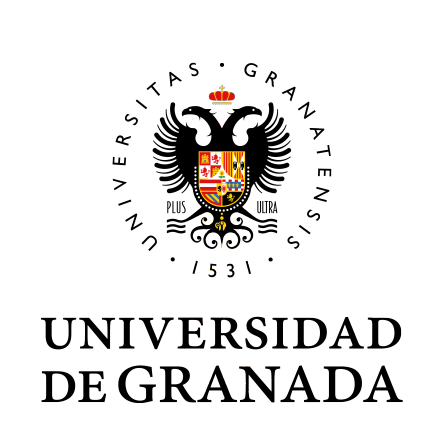
\includegraphics[scale=0.5]{img/ugr.png}\\

        \textsc{\Large \asignatura{}\\[0.2cm]}
        \textsc{MÁSTER CIENCIA DE DATOS E INGENIERÍA DE COMPUTADORES}\\[1cm]

        \noindent\rule[-1ex]{\textwidth}{1pt}\\[1.5ex]
        \textsc{{\Huge \titulo\\[0.5ex]}}
        \textsc{{\Large \subtitulo\\}}
        \noindent\rule[-1ex]{\textwidth}{2pt}\\[2.5ex]

        \end{minipage}

        \vspace{0.3cm}

        \begin{minipage}{\textwidth}

        \centering

        \textbf{Autor}\\ {\autor{} \\ ignaciove@correo.ugr.es}\\[1.5ex]
        \vspace{0.4cm}

        
\includegraphics[scale=0.3]{img/etsiit.jpeg}
        
\includegraphics[scale=0.6]{img/master.png}

        \vspace{0.7cm}
        \textsc{Escuela Técnica Superior de Ingenierías Informática y de Telecomunicación}\\
        \vspace{1cm}
        \textsc{Curso 2020-2021}
    \end{minipage}
\end{titlepage}
% ==============================================================================
    
    \pagenumbering{arabic}    
    \newpage

    % ==============================================================================

\section{Experimento}

Para el ejercicio se ha usado un conjunto de tweets extraídos de la API gracias a la consulta \textbf{\#Oscars2021 lang:en}. El resultado obtenido es un conjunto de 977 tweets sobre el cuál se calcula una tag-cloud, un clustering jerárquico y un conjunto de reglas difusas.

\vspace{\baselineskip}

La lista de técnicas utilizadas en el preprocesamiento son:
\begin{enumerate}
    \item Eliminación de URLs y símbolos especiales.
    \item Eliminación de tweets excesivamente cortos.
    \item Filtrado de sustantivos.
    \item Stemming.
\end{enumerate}

\vspace{\baselineskip}

\begin{figure}[H]\center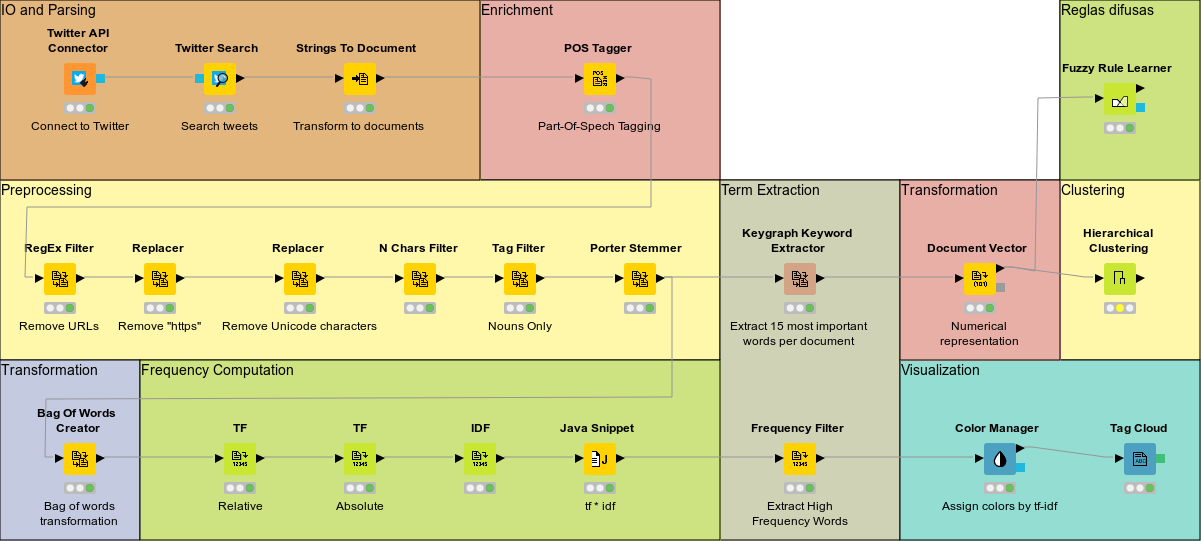
\includegraphics[width=.98\linewidth]{img/workflow.png}\caption{Workflow general del experimento.}\end{figure}

\begin{figure}[H]\center
\includegraphics[width=.8\linewidth]{img/tagCloud.png}\caption{Tag cloud.}\end{figure}

\begin{figure}[H]\center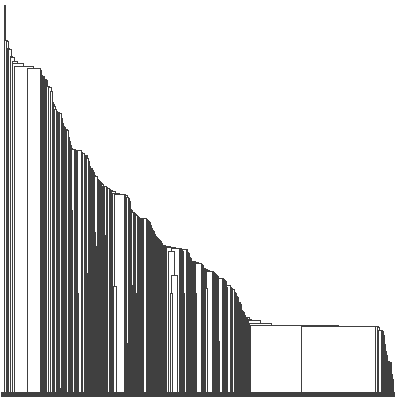
\includegraphics[width=.8\linewidth]{img/dendrograma.png}\caption{Dendrograma del análisis jerárquico.}\end{figure}

\begin{figure}[t]\center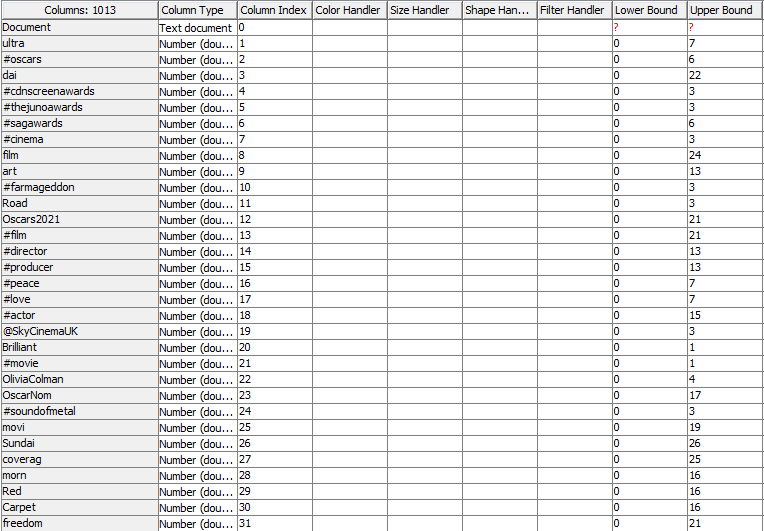
\includegraphics[width=.95\linewidth]{img/clusters.png}\caption{Algunos de los clusters obtenidos.}\end{figure}

\begin{figure}[b]\center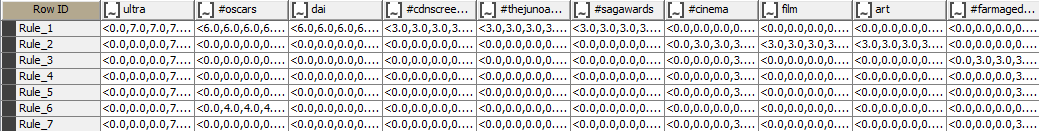
\includegraphics[width=.95\linewidth]{img/reglas.png}\caption{Tabla de reglas.}\end{figure}


% ==============================================================================

    \setlength{\parskip}{1em}
    \newpage
\end{document}

% ==============================================================================
% ==============================================================================